\chapter{Background}\label{chap:Background}

\section{Fundamentals of Graph Theory}

Graph Theory is the study of objects called \textit{vertices} or \textit{nodes} and their relationships which we call \textit{edges}. An edge between vertices $u$ and $v$ is typically denoted $uv$ or $(u,v)$. A graph $G$ is formally defined as an ordered pair $G = (V,E)$ where $V$ is the set of all vertices in $G$ and $E$ is the set of all edges between vertices in $G$. These sets are sometimes refered to as $V(G)$ and $E(G)$, respectively.

$G$ is called a \textit{simple graph} if: (1) there is at most 1 edge between any two vertices, (2) there are no edges from a vertex to itself and (3) all edges have no directionality to them, meaning $uv=vu$ for any edge $uv\in E(G)$. For the rest of this paper all graphs are finite simple graphs, but note that unions and subgraphs are defined the same way for directed graphs and infinite graphs.

Graphs are more intuitive to work with through their visual representations instead of their formal definitions. Let the simple graph $G$ where $V(G)=\{A,B,C,D,E,a,b,c,\newline d, e\}$ and $E(G)=\{Aa,Bb,Cc,Dd,Ee,AB,BC,CD,DE,EA,ac,ce,eb,bd,da\}$. G is often called the \textit{Petersen} graph. It's unwieldy when described formally, yet its visual representation is very easy to understand.

\begin{figure}[H]
\begin{center}
    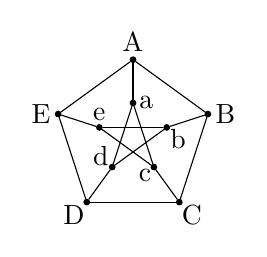
\begin{tikzpicture}[every node/.style={draw, circle, fill=black, minimum size=2pt, inner sep=0pt},scale=1]
    
        % Outer vertices (A,B,C,D,E)
        \node (A0) at (90:1)   [label=above:A] {};
        \node (A1) at (18:1)   [label=right:B] {};
        \node (A2) at (306:1)  [label=below right:C] {};
        \node (A3) at (234:1)  [label=below left:D] {};
        \node (A4) at (162:1)  [label=left:E] {};
    
        % Inner vertices (a,b,c,d,e)
        \node (B0) at (90:0.45)   [label=right:a] {};
        \node (B1) at (18:0.45)   [label=below right:b] {};
        \node (B2) at (306:0.45)  [label=below left:c] {};
        \node (B3) at (234:0.45)  [label=above left: d] {};
        \node (B4) at (162:0.45)  [label=above:e] {};
    
        % Outer edges
        \draw (A0) -- (A1);
        \draw (A1) -- (A2);
        \draw (A2) -- (A3);
        \draw (A3) -- (A4);
        \draw (A4) -- (A0);
    
        % Inner edges
        \draw (B0) -- (B2);
        \draw (B2) -- (B4);
        \draw (B4) -- (B1);
        \draw (B1) -- (B3);
        \draw (B3) -- (B0);
    
        % Spokes
        \draw (A0) -- (B0);
        \draw (A1) -- (B1);
        \draw (A2) -- (B2);
        \draw (A3) -- (B3);
        \draw (A4) -- (B4);
    
    \end{tikzpicture}
\end{center}
    \caption{The Petersen graph}
    \label{fig:petersen graph}
    \end{figure}

We say two graphs $G$ and $H$ are \textit{isomorphic} if there exists a bijection from $V(G)$ to $V(H)$ that induces a bijection from $E(G)$ to $E(H)$ and we denote this relationship via $G\equiv H$. In other words, we consider two graphs $G,H$ to be the 'same' if we can relabel and/or move vertices in some fashion (without adding/removing vertices edges) in a visual representations of $G$ and $H$ to go back and forth between the two.

\begin{figure}[H]
    \begin{center}
    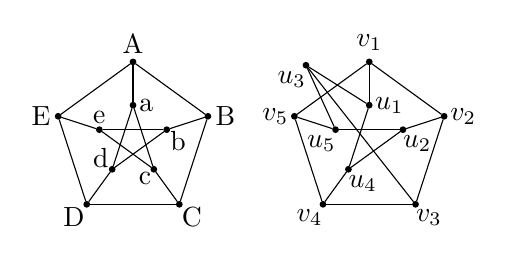
\begin{tikzpicture}[every node/.style={draw, circle, fill=black, minimum size=2pt, inner sep=0pt}]

        % Outer vertices (A,B,C,D,E)
        \node (A0) at (90:1)   [label=above:A] {};
        \node (A1) at (18:1)   [label=right:B] {};
        \node (A2) at (306:1)  [label=below right:C] {};
        \node (A3) at (234:1)  [label=below left:D] {};
        \node (A4) at (162:1)  [label=left:E] {};
    
        % Inner vertices (a,b,c,d,e)
        \node (B0) at (90:0.45)   [label=right:a] {};
        \node (B1) at (18:0.45)   [label=below right:b] {};
        \node (B2) at (306:0.45)  [label=below left:c] {};
        \node (B3) at (234:0.45)  [label=above left: d] {};
        \node (B4) at (162:0.45)  [label=above:e] {};
    
        % Outer edges
        \draw (A0) -- (A1);
        \draw (A1) -- (A2);
        \draw (A2) -- (A3);
        \draw (A3) -- (A4);
        \draw (A4) -- (A0);
    
        % Inner edges
        \draw (B0) -- (B2);
        \draw (B2) -- (B4);
        \draw (B4) -- (B1);
        \draw (B1) -- (B3);
        \draw (B3) -- (B0);
    
        % Spokes
        \draw (A0) -- (B0);
        \draw (A1) -- (B1);
        \draw (A2) -- (B2);
        \draw (A3) -- (B3);
        \draw (A4) -- (B4);

        \begin{scope}[shift={(3,0)}]
            % Outer vertices: v_1 to v_5
            \node (A0) at (90:1)   [label=above:$v_1$] {};
            \node (A1) at (18:1)   [label=right:$v_2$] {};
            \node (A2) at (306:1)  [label=below right:$v_3$] {};
            \node (A3) at (234:1)  [label=below left:$v_4$] {};
            \node (A4) at (162:1)  [label=left:$v_5$] {};

            % Inner vertices: u_1 to u_5
            \node (B0) at (90:0.45)   [label=right:$u_1$] {};
            \node (B1) at (18:0.45)   [label=below right:$u_2$] {};
            \node (B2) at (130:1.25)  [label=below left:$u_3$] {};
            \node (B3) at (234:0.45)  [label=below right:$u_4$] {};
            \node (B4) at (162:0.45)  [label=below left:$u_5$] {};

            % Outer edges (pentagon)
            \draw (A0) -- (A1);
            \draw (A1) -- (A2);
            \draw (A2) -- (A3);
            \draw (A3) -- (A4);
            \draw (A4) -- (A0);

            % Inner edges (star)
            \draw (B0) -- (B2);
            \draw (B2) -- (B4);
            \draw (B4) -- (B1);
            \draw (B1) -- (B3);
            \draw (B3) -- (B0);

            % Spokes between outer and inner
            \draw (A0) -- (B0);
            \draw (A1) -- (B1);
            \draw (A2) -- (B2);
            \draw (A3) -- (B3);
            \draw (A4) -- (B4);
        \end{scope}

    \end{tikzpicture}
\end{center}
    \caption{$G\cong H$}
    \label{fig:isomorphismexample}

\end{figure}

Graph theorists casually refer to two graphs as the 'same' graph if they are in the same isomorphism class. We will wrap up the fundamentals with a few mdefinitions and some algebraic tools.

\begin{definition}[Subgraph] A subgraph $G\subseteq K$ is a graph whose vertices and edges are subsets of the vertices and edges of $K$; $G\subseteq K$ if $V(G)\subseteq V(K)$ and $E(G)\subseteq E(K)$.
\end{definition}


\begin{definition}[Vertex-induced Subgraph] A \textit{vertex-induced} subgraph $G\subseteq K$ is one whose vertices are some subset of $V(K)$ and whose edges are all edges between those vertices in $K$; $V(G)\subseteq V(K)$ and $E(G)=\{uv\in E(K)\mid u,v\in E(G)\}$. If $G$ is such a subgraph we say that $G$ is induced by $S=V(G)\subseteq V(K)$.
\end{definition}

\begin{definition}[Edge-induced Subgraph] A \textit{edge-induced} subgraph $G\subseteq K$ is one whose edges are some subset of $E(K)$ and whose vertices are all those who appear as an endpoint in that subset of edges; $E(G)\subseteq E(K)$ and $V(G)=\{v\in V(K)\mid vu\in E(G) \text{or }uv\in E(G)\text{ for some }u\in V(K)\}$. If $G$ is such a subgraph we say that $G$ is induced by $S=E(G)\subset E(K)$
\end{definition}

Here is a visual example of these types of graphs: Let $K$ be the Petersen graph from Figure \ref{fig:petersen graph}. Now, let
\begin{align*}
    &\textbf{Subgraph: } \textcolor{magenta}{G} \subseteq K \text{ where }\textcolor{magenta}{V(G)} = \textcolor{magenta}{\{E, e, b\}},\; \textcolor{magenta}{E(G)} = \textcolor{magenta}{\{Ee\}}.\\
    &\textbf{Vertex-induced Subgraph: } \textcolor{blue}{H} \subseteq K \text{ is induced by } \textcolor{blue}{\{a, A, B\}}\subseteq V(K)\\
    &\textbf{Edge-induced Subgraph: } \textcolor{red}{M} \subseteq K 
    \text{ is induced by }\textcolor{red}{\{Dd, DC, Cc\}}\subseteq E(K)
\end{align*}
The figure below shows $K$ and it's color-coded subgraphs.

\begin{figure}[H]
    \begin{center}
    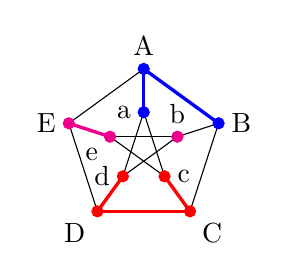
\begin{tikzpicture}[scale=1]
    
        %--- Base style for all nodes:
        \tikzstyle{base node}=[draw, circle, fill=black, minimum size=2pt, inner sep=0pt]
    
        %--- Outer vertices (A,B,C,D,E)
        \node[base node, label=above:A]         (A0) at (90:1)   {};
        \node[base node, label=right:B]         (A1) at (18:1)   {};
        \node[base node, label=below right:C]   (A2) at (306:1)  {};
        \node[base node, label=below left:D]    (A3) at (234:1)  {};
        \node[base node, label=left:E]          (A4) at (162:1)  {};
    
        %--- Inner vertices (a,b,c,d,e)
        \node[base node, label=left:a]         (B0) at (90:0.45)   {};
        \node[base node, label=above:b]   (B1) at (18:0.45)   {};
        \node[base node, label=right:c]    (B2) at (306:0.45)  {};
        \node[base node, label=left:d]    (B3) at (234:0.45)  {};
        \node[base node, label=below left:e]         (B4) at (162:0.45)  {};
    
        %--- Edges of K (in black)
        % Outer ring
        \draw (A0) -- (A1);
        \draw (A1) -- (A2);
        \draw (A2) -- (A3);
        \draw (A3) -- (A4);
        \draw (A4) -- (A0);
    
        % Inner pentagon
        \draw (B0) -- (B2);
        \draw (B2) -- (B4);
        \draw (B4) -- (B1);
        \draw (B1) -- (B3);
        \draw (B3) -- (B0);
    
        % Spokes
        \draw (A0) -- (B0);
        \draw (A1) -- (B1);
        \draw (A2) -- (B2);
        \draw (A3) -- (B3);
        \draw (A4) -- (B4);
    
        %=== Subgraph G in magenta: V(G)={E, e, b}, E(G)={Ee, eb}
        \draw[magenta, very thick] (A4) -- (B4);  % E--e
        %\draw[magenta, very thick] (B4) -- (B1);  % e--b
        \node[draw=magenta, fill=magenta, circle, minimum size=4pt, inner sep=0pt] at (A4) {};
        \node[draw=magenta, fill=magenta, circle, minimum size=4pt, inner sep=0pt] at (B4) {};
        \node[draw=magenta, fill=magenta, circle, minimum size=4pt, inner sep=0pt] at (B1) {};
    
        %=== Vertex-induced subgraph H in blue: induced by {a, A, B}
        % Edges among {a,A,B} in K are A--B and A--a
        \draw[blue, very thick] (A0) -- (A1);   % A--B
        \draw[blue, very thick] (A0) -- (B0);   % A--a
        \node[draw=blue, fill=blue, circle, minimum size=4pt, inner sep=0pt] at (A0) {};
        \node[draw=blue, fill=blue, circle, minimum size=4pt, inner sep=0pt] at (A1) {};
        \node[draw=blue, fill=blue, circle, minimum size=4pt, inner sep=0pt] at (B0) {};
    
        %=== Edge-induced subgraph M in red: induced by {Dd, DC, Cc}
        % These edges correspond to D--d, D--C, C--c in K
        \draw[red, very thick] (A3) -- (B3);    % D--d
        \draw[red, very thick] (A3) -- (A2);    % D--C
        \draw[red, very thick] (A2) -- (B2);    % C--c
        \node[draw=red, fill=red, circle, minimum size=4pt, inner sep=0pt] at (A3) {};
        \node[draw=red, fill=red, circle, minimum size=4pt, inner sep=0pt] at (B3) {};
        \node[draw=red, fill=red, circle, minimum size=4pt, inner sep=0pt] at (A2) {};
        \node[draw=red, fill=red, circle, minimum size=4pt, inner sep=0pt] at (B2) {};
    
    \end{tikzpicture}
    \end{center}
    \caption{$K$ and subgraphs $\textcolor{magenta}{G}, \textcolor{blue}{H}, \textcolor{red}{M} \subseteq K$}
    \label{fig:subgraphs}
    \end{figure}
Next, we will talk about two important operations done on graphs.

\begin{definition}[Graph Union]
The union of two graphs $G$ and $H$ is simply the graph resulting from the union of their vertices and the union of their edges and is denoted $G\cup H$; $G\cup H=(V(G)\cup V(H),E(G)\cup E(H))$. If $G$ and $H$ are edge-disjoint, we denote their union via $G\sqcup H$ and call it a \textit{disjoint union} of $G$ and $H$.
\end{definition}

Here is an example of a union and a disjoint union of graphs. Let $G=(\{a,b,c,d\},\{ab,\newline bc,cd,da\}),H=(\{a,b,c\},\{ab,bc,ca\}),\text{ and }K=(\{A,B,C\},\{AB,BC,CA\})$ Then:
\begin{align*}
&G\cup H = (\{a,b,c,d\},\{ab,bc,cd,da,ca\})\\
&G\sqcup K=V(G\sqcup K)=(\{a,b,c,d,A,B,C\},\{ab,bc,cd,da,AB,BC,CA\})
\end{align*}
These unions are depicted in the following figure.
\begin{figure}[H]
    \begin{center}
        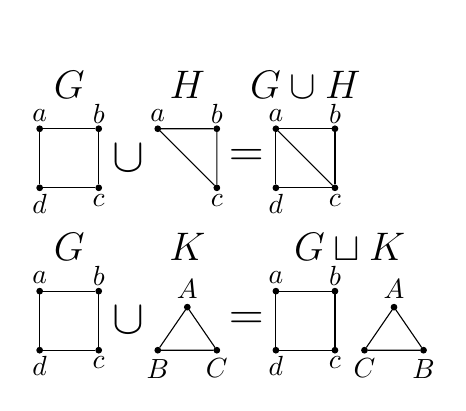
\begin{tikzpicture}[every node/.style={draw, circle, fill=black, minimum size=2pt, inner sep=0pt},scale=0.75]
            \node(G) at (0.5,0.75) [draw=none, fill=none] {\Large $G$};
            % First graph
            \node (a) at (0, 0)  [label=above:$a$]  {};
            \node (b) at (1, 0)  [label=above:$b$]  {};
            \node (c) at (1, -1) [label=below:$c$]  {};
            \node (d) at (0, -1) [label=below:$d$]  {};

            \draw (a) -- (b) -- (c) -- (d) -- (a);

            % "=" symbol
            \node[draw=none, fill=none] at (1.5, -0.5) {\LARGE $\cup$};

            % Second graph
            \begin{scope}[xshift=2cm]
                \node(H) at (0.5,0.75) [draw=none, fill=none] {\Large $H$};
                \node (a) at (0, 0)  [label=above:$a$]  {};
                \node (b) at (1, 0)  [label=above:$b$]  {};
                \node (c) at (1, -1) [label=below:$c$]  {};
    
                \draw (a) -- (b) -- (c) -- (a);
            \end{scope}

            % "\cup" symbol
            \node[draw=none, fill=none] at (3.5, -0.5) {\LARGE $=$};
            
            \begin{scope}[xshift=4cm]
                \node(GUH) at (0.5,0.75) [draw=none, fill=none] {\Large $G\cup H$};
                \node (a) at (0, 0)  [label=above:$a$]  {};
                \node (b) at (1, 0)  [label=above:$b$]  {};
                \node (c) at (1, -1) [label=below:$c$]  {};
                \node (d) at (0, -1) [label=below:$d$]  {};
    
                \draw (a) -- (b) -- (c) -- (d) -- (a);
                \draw (a) -- (c);
            \end{scope}

%second line _______________________________________________________

            \begin{scope}[shift={(0,-2.75)}]
                            % First graph
                            \node(G) at (0.5,0.75) [draw=none, fill=none] {\Large $G$};
                            \node (a) at (0, 0)  [label=above:$a$]  {};
                            \node (b) at (1, 0)  [label=above:$b$]  {};
                            \node (c) at (1, -1) [label=below:$c$]  {};
                            \node (d) at (0, -1) [label=below:$d$]  {};

                            \draw (a) -- (b) -- (c) -- (d) -- (a);

                            % "=" symbol
                            \node[draw=none, fill=none] at (1.5, -0.5) {\LARGE $\cup$};
            \end{scope}

            % Second graph
            \begin{scope}[shift={(2,-2.75)}]
                % Define coordinates so the sides are all length 2.
                \node(K) at (0.5,0.75) [draw=none, fill=none] {\Large $K$};
                \node (A) at (0.5,-0.271) [label=above:$A$]{};
                \node (B) at (0,-1) [label=below:$B$]{};
                \node (C) at (1,-1) [label=below:$C$] {};

                % Draw and label
                \draw (A) -- (B) -- (C) -- (A);
                \node[draw=none, fill=none] at (1.5, -0.5) {\LARGE $=$};
            \end{scope}

            \begin{scope}[shift={(4,-2.75)}]
                \node(GUH) at (1.25,0.75) [draw=none, fill=none] {\Large $G\sqcup K$};
                \node (a) at (0, 0)  [label=above:$a$]  {};
                \node (b) at (1, 0)  [label=above:$b$]  {};
                \node (c) at (1, -1) [label=below:$c$]  {};
                \node (d) at (0, -1) [label=below:$d$]  {};

                \node (A) at (2,-0.271) [label=above:$A$]{};
                \node (B) at (2.5,-1) [label=below:$B$]{};
                \node (C) at (1.5,-1) [label=below:$C$] {};

                \draw (a) -- (b) -- (c) -- (d) -- (a);
                \draw (A) -- (B) -- (C) -- (A);
            \end{scope}

        \end{tikzpicture}
    \end{center}
    \caption{(above)$\,G\cup H$ and (below)$\,G\sqcup K$}
    \label{fig:unions}
\end{figure}

Next, we define another very important operation that combines two graphs in a different manner.

\begin{definition}[Join]
    Let $G$ and $H$ be vertex disjoint graphs. Their
    \textit{join}, denoted via $G \vee H$, is the graph obtained by
    taking the disjoint union of $G$ and $H$ and adding all
    possible edges between every vertex in $G$ and every vertex
    in $H$. Formally:
    $$
      G \vee H
      \;=\;
      \bigl(
        V(G)\cup V(H),
        E(G)\;\cup\;E(H)\;\cup\;\{\,xy \mid x\in V(G),\, y\in V(H)\}
      \bigr).
    $$
  \end{definition}
Here is an example. Let $G=(\{a,b,c\},\{ab,bc,ca\})$ and $H=(\{A,B,C\},\{AB,BC,CA\})$, then $G\lor H=(\{a,b,c,A,B,C\},E(G)\sqcup E(H)\sqcup\{aA,aB,aC,bA,bB,bC,cA,cB,cC\})$. This join is depicted in the figure below.

\begin{figure}[H]
    \begin{center}
        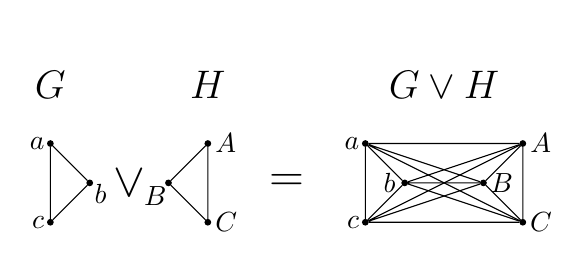
\begin{tikzpicture}[every node/.style={draw, circle, fill=black, minimum size=2pt, inner sep=0pt},scale=1]
            \node (G) at (0,0.75) [draw=none, fill=none] {\Large $G$};
            \node (a) at (0,0) [label=left:$a$]{};
            \node (b) at (0.5,-0.5) [label=below right:$b$]{};
            \node (c) at (0,-1) [label=left:$c$]{};

            \draw (a) -- (b) -- (c) -- (a) {};

            \node[draw=none, fill=none] at (1, -0.5) {\LARGE $\lor$};

            \node (H) at (2,0.75) [draw=none, fill=none] {\Large $H$};
            \node (A) at (2,0) [label = right:$A$]{};
            \node (B) at (2,-1)[label = right:$C$]{};
            \node (C) at (1.5,-0.5) [label = below left:$B$]{};

            \draw(A) -- (B) -- (C) -- (A){};

            \node[draw=none, fill=none] at (3, -0.5) {\LARGE $=$};

            \begin{scope}[shift={(4,0)}]
                \node (GVH) at (1,0.75) [draw=none, fill=none] {\Large $G\lor H$};
                \node (a) at (0,0) [label=left:$a$]{};
                \node (b) at (0.5,-0.5) [label=left:$b$]{};
                \node (c) at (0,-1) [label=left:$c$]{};

                \draw (a) -- (b) -- (c) -- (a) {};

                \node (A) at (2,0) [label = right:$A$]{};
                \node (B) at (2,-1)[label = right:$C$]{};
                \node (C) at (1.5,-0.5) [label = right:$B$]{};

                \draw(A) -- (B) -- (C) -- (A){};

                \draw (a) -- (A) -- (a) -- (B) -- (a) -- (C);
                \draw (b) -- (A) -- (b) -- (B) -- (b) -- (C);
                \draw (c) -- (A) -- (c) -- (B) -- (c) -- (C);
            \end{scope}
        \end{tikzpicture}
    \end{center}
    \caption{(above)$\,G\cup H$ and (below)$\,G\sqcup K$}
    \label{fig:join}
\end{figure}

Lastly, we define a few characteristics of graphs and their components. These may or may not be used frequently in this paper, but are important concepts to know in order to be able to talk about graphs comfortably.

Let $G$ be a simple graph. We say two vertices $u,v\in V(G)$ are \textit{adjacent} or \textit{neighbors} if they share an edge $uv\in E(G)$. Similarly, we say a vertex is \textit{incident} with an edge if it is one of it's endpoints; $u\in V(G)$ is incident with $e\in E(G)$ if $e=uv$ for some $v\in V(G)$. The set of all vertices adjacent to $u$ in $G$  is called the \textit{neighborhood} of $v$ denoted $N_{G}(v)$ or simply $N(v)$. Sometimes this is refered to as the open neighborhood of $v$ in $G$ and then the closed neighborhood is defined via $N_{G}[v]=N_{G}(v)\cup \{v\}$. The \textit{degree} of a vertex $v\in V(G)$ is the number of vertices adjacent to it and is denoted via $deg_{G}(v)=|N_{G}(v)|$ or simply $deg(v)$. Equivalently, the degree is the number or edges incident to it or the number of neighbors that $G$ has.

The following are three similar types of objects we can form from graphs.

\begin{definition}[Walk]
Let $G$ be a graph on $n$ vertices. A \textit{walk} in $G$ is a sequence $(w_{0},w_{1},\hdots,w_{k})$ of vertices in $G$ whose adjacent elements must be adjacent in $G$. Adjacent elements in a walk much be distinct vertices but a vertex may be repeated multiple times.
\end{definition}

\begin{definition}[Path]
Let $G$ be a graph on $n$ vertices. A \textit{path} in $G$ is a sequence $(v_{0},v_{1},\hdots,v_{k})$ of distinct vertices in $G$ whose adjacent elements must be adjacent in $G$, and where no vertex is repeated. This sequence gives the subgraph of $G$ induced by $\{v_{0}v_{1},v_{1}v_{2},\hdots,v_{k-1}v_{k}\}$.
\end{definition}

\begin{definition}[Cycle]
Let $G$ be a graph on $n$ vertices. A \textit{cycle} in $G$ is a sequence $(v_{0},v_{1},\hdots,v_{k},v_{0})$ of internally distinct vertices (distinct except on the endpoints) that begins and terminates at the same vertex $v_{0}$. Often such a cycle is denoted via $(v_{0}v_{1}\cdots v_{k})$ and it is understood that the sequence wraps back around to $v_{0}$ after $v_{k}$. Additionally, the cycle $(v_{0}v_{1}\cdots v_{k})$ is equivalent to $(v_{1}\cdots v_{k}v_{0})$, $(v_{2}\cdots v_{k}v_{0}v_{1}),\hdots$ and so on. 
\end{definition}

let $G$ be a simple graph. We call $G$ \textit{acyclic} if it contains no cycles. If there exists a path from any vertex to every other vertex in $G$, then we call $G$ \textit{connected}. If not, we call $G$ \textit{disconnected}. We call the set of connected subgraphs of $G$ whose disjoint union equals $G$ the \textit{connected components} of $G$.

This concludes the fundamental concepts needed to understand this project. The next and final section of this chapter will introduce all the fundamental families of graphs we refer to in the proceeding chapters.

\section{Fundamental Families of Graphs}

In this section introduce some fundamental families of graphs which we refer to throughout this paper. Often instead of fully defining the graphs being worked with, we simply refer to it as a member of a larger family of graphs. These families are not completely distinct, but sometimes it is helpful to view graphs as a member of one family or another depending on the context.

Recall that a graph is acyclic if it contains no cycles. Similarly, we call a graph \textit{$k$-cyclic} if it contains exactly $k$ distinct cycles. If $k=2\text{ or }3$ we call it \textit{bicyclic} or \textit{tricyclic}, respectively. In a similar vein, we call a graph \textit{$k$-partite} if we can partition it's vertices into $k$ disjoint sets.If $k=2\text{ or }3$, we call it \textit{bipartite} or \textit{tripartite}, respectively. These are all very broad families of graphs often used to characterize graphs within another family. The following are more nuanced, and more popular families of graphs to work with.

\begin{definition}[Complete Graph]
    The \textit{complete graph} on $n$ vertices, denoted $K_n$, is the
    graph on $n$ vertices such that every pair of distinct vertices shares an edge.
\end{definition}

\begin{figure}[H]
    \begin{center}
    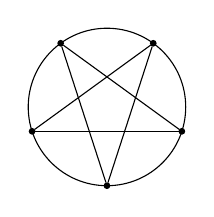
\begin{tikzpicture}[scale=1, every node/.style={draw, circle, fill=black, minimum size=2pt, inner sep=0pt}]
    
    % Draw the circle outline (optional, you may comment it out if you don't want it visible)
    \draw[black] (0,0) circle (1);
    
    % Place nodes on the circle. We use angles so that the pentagon is rotated with the bottom vertex at 270°.
    \node (A) at (270:1) {};   % bottom
    \node (B) at (342:1) {};   % lower right
    \node (C) at (54:1)  {};   % upper right
    \node (D) at (126:1) {};   % upper left
    \node (E) at (198:1) {};   % lower left
    
    % Draw the outer cycle edges as arcs along the circle
    %\draw (A) arc (270:342:1);
    %\draw (B) arc (342:54:1);
    %\draw (C) arc (54:126:1);
    %\draw (D) arc (126:198:1);
    %\draw (E) arc (198:270:1);
    
    % Draw the remaining edges (the diagonals) as straight lines to complete K_5
    \draw (A) -- (C);
    \draw (A) -- (D);
    \draw (B) -- (D);
    \draw (B) -- (E);
    \draw (C) -- (E);
    
    \end{tikzpicture}
    \end{center}
    \caption{The Complete Graph $K_{5}$}
    \label{fig:K5}
    \end{figure}
  
\begin{definition}[Complete Bipartite Graph]
    Let $m,n\in \NN$. The \textit{complete bipartite graph} $K_{m,n}$ is the bipartite graph whose vertices can be partitioned into two disjoint sets of sizes $m$ and $n$, respectively, such that every vertex in the one partite set is adjacent to every vertex in the other partite set and there no edges between vertices in the same partite set.
\end{definition}

\begin{figure}[H]
    \begin{center}
        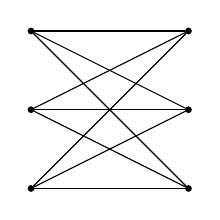
\begin{tikzpicture}[every node/.style={draw, circle, fill=black, minimum size=2pt, inner sep=0pt}, scale=1]
            % Left partite set
            \node (A1) at (0,2) {};
            \node (A2) at (0,1) {};
            \node (A3) at (0,0) {};
            
            % Right partite set
            \node (B1) at (2,2) {};
            \node (B2) at (2,1) {};
            \node (B3) at (2,0) {};
            
            % Edges between the two partite sets
            \draw (A1) -- (B1);
            \draw (A1) -- (B2);
            \draw (A1) -- (B3);
            
            \draw (A2) -- (B1);
            \draw (A2) -- (B2);
            \draw (A2) -- (B3);
            
            \draw (A3) -- (B1);
            \draw (A3) -- (B2);
            \draw (A3) -- (B3);
        \end{tikzpicture}
    \end{center}
    \caption{The Complete Bipartite Graph \( K_{3,3} \)}
    \label{fig:complete_bipartite_k33}
    \end{figure}
    
  
\begin{definition}[Complete Multipartite Graph]
The \textit{complete $k$-partite graph} or \textit{complete multipartite graph} $K_{n_1,\,\dots,\,n_k}$ is the graph whose vertices can be partitioned into $k$ disjoint sets of sizes $n_1,\,n_2,\,\hdots,\,n_k$, respectively such that such that every vertex in the one partite set is adjacent to every vertex in the other $k-1$ partite sets and there no edges between vertices in the same partite set.

If all partite sets are the same size $n$ we call this graph the \textit{complete equipartite graph} $K_{n:k}$ or $K_{n\times m}$.
\end{definition}

\begin{figure}[H]
    \begin{center}
    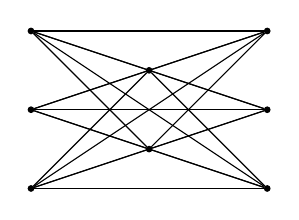
\begin{tikzpicture}[every node/.style={draw, circle, fill=black, minimum size=2pt, inner sep=0pt}, scale=1]
    
    % Partite set A (3 nodes)
    \node (A1) at (0,1) {};
    \node (A2) at (0,0) {};
    \node (A3) at (0,-1) {};
    
    % Partite set B (2 nodes)
    \node (B1) at (1.5,0.5) {};
    \node (B2) at (1.5,-0.5) {};
    
    % Partite set C (3 nodes)
    \node (C1) at (3,1) {};
    \node (C2) at (3,0) {};
    \node (C3) at (3,-1) {};
    
    % Edges between A and B
    \foreach \i in {1,2,3} {
        \foreach \j in {1,2} {
            \draw (A\i) -- (B\j);
        }
    }
    
    % Edges between A and C
    \foreach \i in {1,2,3} {
        \foreach \j in {1,2,3} {
            \draw (A\i) -- (C\j);
        }
    }
    
    % Edges between B and C
    \foreach \i in {1,2} {
        \foreach \j in {1,2,3} {
            \draw (B\i) -- (C\j);
        }
    }
    
    \end{tikzpicture}
    \end{center}
    \caption{The Complete Multipartite Graph \( K_{3,2,3} \)}
    \label{fig:complete_multipartite_k323}
    \end{figure}
       

\begin{definition}[Cycle Graph]
The \textit{cycle graph} on $n$ vertices denoted $C_{n}$ is a graph with exactly one cycle containing all of it's edges.
\end{definition}

\begin{figure}[H]
    \begin{center}
    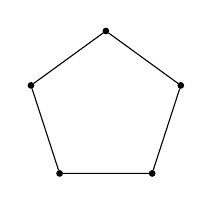
\begin{tikzpicture}[every node/.style={draw, circle, fill=black, minimum size=2pt, inner sep=0pt}, scale=1]
        % Place vertices to form an upward-facing pentagon
        \node (v1) at (90:1)   {};   % Top vertex
        \node (v2) at (18:1)   {};
        \node (v3) at (306:1)  {};
        \node (v4) at (234:1)  {};
        \node (v5) at (162:1)  {};
        
        % Connect vertices in cyclic order to form the pentagon (cycle graph C_5)
        \draw (v1) -- (v2) -- (v3) -- (v4) -- (v5) -- (v1);
    \end{tikzpicture}
    \end{center}
    \caption{The Cycle Graph \( C_5 \)}
    \label{fig:C5-up}
    \end{figure}

\begin{definition}[Tree]
A \textit{tree} is any connected acyclic graph. Trees on $n$ vertices have $n-1$ edges. Equivalently, these graphs are any connected bipartite graphs.
\end{definition}

\begin{figure}[H]
    \begin{center}
    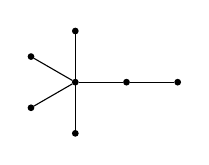
\begin{tikzpicture}[scale=1.3,
      every node/.style={draw, circle, fill=black, minimum size=2pt, inner sep=0pt}
    ]
    
    \node (G1N2) at (210:0.5) {};
    \node (G1N0) at (0:0) {};
    \node (G1N1) at (0:0.5) {};
    \node (G1N6) at (0:1) {};
    \node (G1N3) at (150:0.5) {};
    \node (G1N4) at (270:0.5) {};
    \node (G1N5) at (90:0.5) {};

    \draw (G1N0) -- (G1N1);
    \draw (G1N0) -- (G1N2);
    \draw (G1N0) -- (G1N3);
    \draw (G1N0) -- (G1N4);
    \draw (G1N0) -- (G1N5);
    \draw (G1N1) -- (G1N6);
    
    \end{tikzpicture}
    \end{center}
    \caption{A Tree Graph on 6 vertices}
    \label{fig:tree_lobster_style}
    \end{figure}
    
\begin{definition}[Path Graph]
The \textit{path} graph on $n$ vertices, denoted $P_n$, is an acyclic graph with exactly one path containing all of it's edges. All paths are trees.
\end{definition}

\begin{figure}[H]
    \begin{center}
    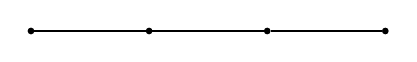
\begin{tikzpicture}[every node/.style={draw, circle, fill=black, minimum size=2pt, inner sep=0pt}, scale=1]
    
    % Place the 4 vertices in a line
    \node (v1) at (0,0) {};
    \node (v2) at (1.5,0) {};
    \node (v3) at (3,0) {};
    \node (v4) at (4.5,0) {};
    
    % Draw edges between consecutive nodes
    \draw (v1) -- (v2) -- (v3) -- (v4);
    
    \end{tikzpicture}
    \end{center}
    \caption{The Path Graph \( P_4 \)}
    \label{fig:path-p4}
    \end{figure}

\begin{definition}[Star Graph]
The \textit{star graph} on $n+1$ vertices, denoted $K_{1,n}$ (or $S_{n+1}$ which we never use in this paper) consisting of one central \textit{hub} vertex adjacent to $n$ \textit{outer} vertices, with no other edges. All stars are trees. Sometimes this graph is refered to as an \textit{n-star}.
\end{definition}

\begin{figure}[H]
    \begin{center}
    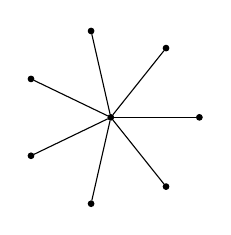
\begin{tikzpicture}[scale=0.75,
      every node/.style={draw, circle, fill=black, minimum size=2pt, inner sep=0pt}
    ]
    
    % Central hub
    \node (C) at (0,0) {};
    
    % Outer nodes evenly spaced in a circle
    \foreach \i in {1,...,7} {
      \node (L\i) at ({360/7 * (\i - 1)}:1.5) {};
      \draw (C) -- (L\i);
    }
    
    \end{tikzpicture}
    \end{center}
    \caption{The $7$-star (\(K_{1,7}\))}
    \label{fig:star-7}
    \end{figure}
    

\begin{definition}[Forest Graph]

Any disjoint union of tree graphs is called a \textit{forest} graph. These graphs are all bipartite and can be equivalently defined as disconnected bipartite graphs.
\end{definition}

\begin{figure}[H]
    \begin{center}
    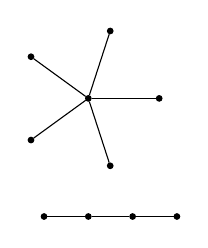
\begin{tikzpicture}[scale=0.75,
      every node/.style={draw, circle, fill=black, minimum size=2pt, inner sep=0pt}
    ]
    
    % Star graph (centered at 0,0)
    \node (C) at (0,0) {};
    \foreach \i in {1,...,5} {
      \node (S\i) at ({360/5 * (\i - 1)}:1.2) {};
      \draw (C) -- (S\i);
    }
    
    % Path of length 2 below the star
    \node (P1) at (-0.75,-2) {};
    \node (P2) at (0,-2) {};
    \node (P3) at (0.75,-2) {};
    \node (P4) at (1.5,-2) {};
    \draw (P1) -- (P2) -- (P3) -- (P4);
    
    \end{tikzpicture}
    \end{center}
    \caption{A forest on 9 vertices}
    \label{fig:star-and-path}
    \end{figure}
    

\begin{definition}[Galaxy Graph]
    Any disjoint union of star graphs is called a \textit{galaxy} graph. We refer to $G=G_{1}\sqcup \cdot \sqcup G_{k}$ as a \textit{$(G_{1},\hdots,G_{k})$-galaxy} graph if $G_{1},\hdots,G_{k}$ are all stars. This family is a subset of the forest family.
\end{definition}

\begin{figure}[H]
    \begin{center}
    \begin{tikzpicture}[scale=1,
      every node/.style={draw, circle, fill=black, minimum size=2pt, inner sep=0pt}
    ]
    
    % 5-edge star (shifted closer to center)
    \node (C1) at (-1.7,0) {};
    \node (A1) at (-1.7,1.2) {};
    \node (A2) at (-2.6,0.6) {};
    \node (A3) at (-2.6,-0.6) {};
    \node (A4) at (-1.7,-1.2) {};
    \node (A5) at (-0.8,0) {};
    
    \draw (C1) -- (A1);
    \draw (C1) -- (A2);
    \draw (C1) -- (A3);
    \draw (C1) -- (A4);
    \draw (C1) -- (A5);
    
    % 6-edge star (shifted closer to center)
    \node (C2) at (1.7,0) {};
    \node (B1) at (1.7,1.2) {};
    \node (B2) at (2.6,0.6) {};
    \node (B3) at (2.6,-0.6) {};
    \node (B4) at (1.7,-1.2) {};
    \node (B5) at (0.8,-0.6) {};
    \node (B6) at (0.8,0.6) {};
    
    \draw (C2) -- (B1);
    \draw (C2) -- (B2);
    \draw (C2) -- (B3);
    \draw (C2) -- (B4);
    \draw (C2) -- (B5);
    \draw (C2) -- (B6);
    
    \end{tikzpicture}
    \end{center}
    \caption{The $(K_{1,6},K_{1,7})$-Galaxy}
    \label{fig:galaxy_close}
    \end{figure}
    
We have now defined a few important families of graphs which we will refer to throughout the rest of this paper. We generally don't explicitly define every graph by its vertices and edges and simply refer to it as some member of one family or say this it is isomorphic to one. This is much more efficient and concise than listing out all vertices and edges as we did in the beginning of this chapter.

We are now ready to move on and introduce graph decompositions, the objects which are the subject of this project.
  














